\section{Partially observable environments and Bayesian methods}
\label{sec:partially_observable}
\textit{This section reviews the lecture slides 13.}
\begin{itemize}
	\item Until now, we always assumed to have a fully observable environment. However, this is often not the case, also in real life (we cannot see what is happening behind walls, or 1000km away. Thus we are \textit{living} in a partially observable environment).
	
	This can happen if we have state aliasing (we see twice the same state although if it would be fully observed, it is clear that we are in two different states), or even simple noise.
	\item First, let's consider a generalization of our environment. We define a latent state in the environment $x'_t$ which captures all information about the true state. From this latent state, we can make an observation $o_t$ per state, which can be seen as measurement of an unknown quantity.
	
	Note that in fully observable environments, we have $s_t=o_t=x'_t$.
	\item A simple approach would be to consider an observation $o_t$ as features from the latent state, and hence use approaches from Section~\ref{sec:value_based_approximation}. But this is usually not sufficient.
	\item In most environments, we can infer information about the latent space by looking at the history $H_t=A_0,O_1,A_1,...,A_{t-1},O_t$, and we choose our next action based on the whole history $A_t=\pi(H_t)$
	\item However, using a full history is neither efficient nor practical (increases in size over time). Hence, we better use a lower dimensional feature representation of the history, $f(H_t)$, and use this as internal state of the policy $s_t = f(H_t)$ (note that $s_t$ has slightly different meaning here because it is the state which the policy sees, not what we get back from the environment).
	\item The best function $f$ would be the one that summarizes all important information. We can define what this means as follows:
	$$f(H_t)=f(H'_t)\implies \Prob{O_{t+1}=o|H=H_t,A_t=a}=\Prob{O_{t+1}=o|H=H'_t,A_t=a}$$
	which means in textual form: if the representation of two histories are the same, then the expectation of the next observation is the same for both histories. Hence, we would also choose the same action, which leads to the conclusion, that the optimal policy can be found solely on $f$.
	
	A function that fulfills this condition is called \textit{Markov function}. For any function which is not Markovian, we can only find an approximate optimal policy, but often not the optimal itself.
	\item Which function is Markovian depends highly on the environment, and will be discussed next.
\end{itemize}
\subsection{Markov functions and histories}
\begin{itemize}
	\item First, let's consider what we need to deal with a partially observable environment. Besides the environment and our policy-/value-based approach, we also have a state-update function (see Figure~\ref{fig:rl_partially_observability_architecture}). Our goal is to find a state-update function which is Markovian and efficient/compact.
	
	\begin{figure}[ht!]
		\centering
		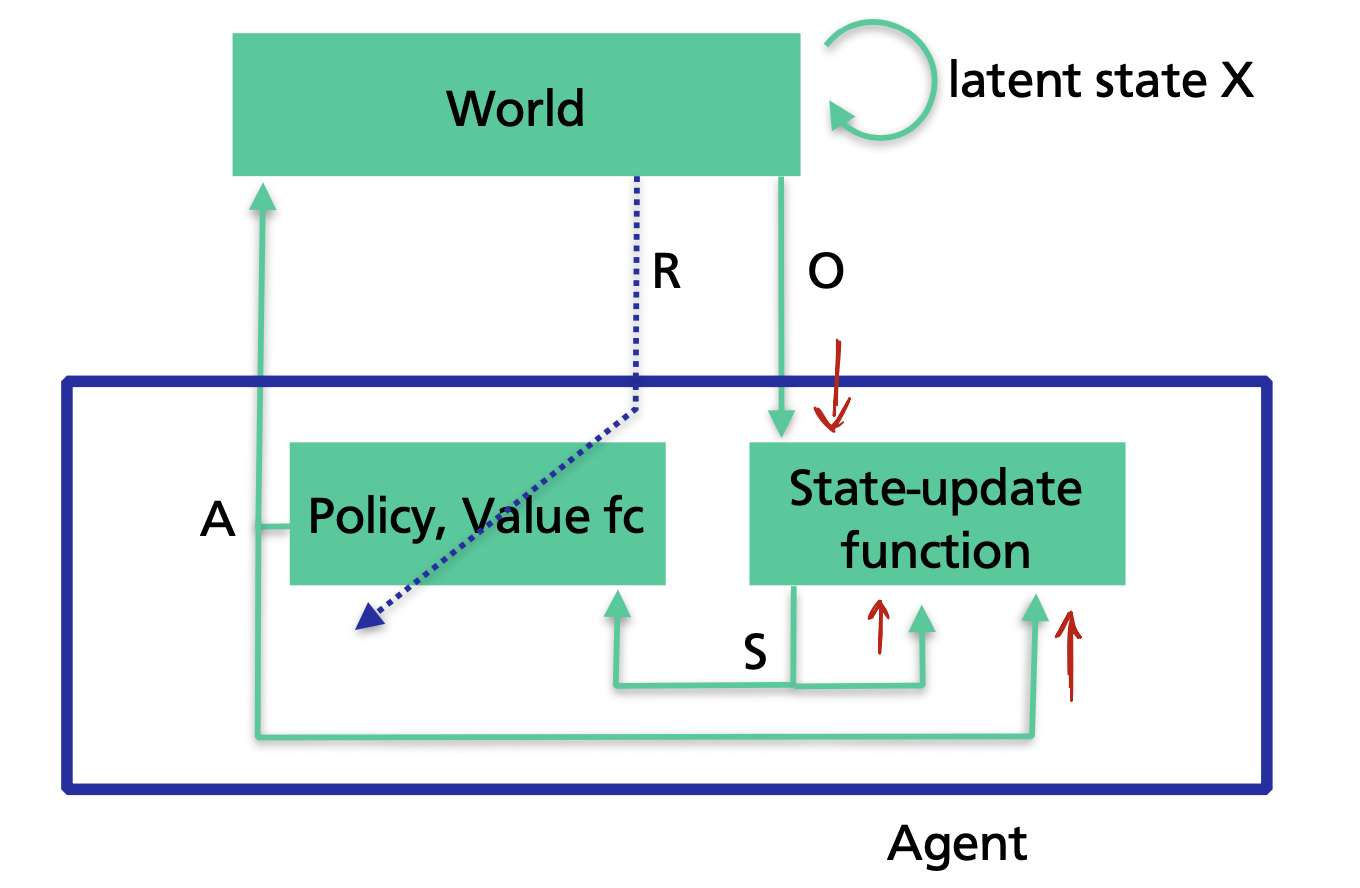
\includegraphics[width=0.5\textwidth]{figures/rl_partially_observability_architecture.png}
		\caption{Overview of the dynamics in dealing with a partially observable environment.}
		\label{fig:rl_partially_observability_architecture}
	\end{figure}
\end{itemize}
\subsubsection{Sample Markov functions}
\begin{itemize}
	\item The simplest function is the identity, meaning $s_t=H_t$. However, this is neither compact, nor can we use it in any tabular policy setting efficiently (all possible sequences must be stored).
	\item We can define an probability distribution over the latent space $X$, and try to do Bayesian inference (i.e. finding the posterior). This is done by calculating a \textbf{belief state}:
	\begin{equation*}
		\begin{split}
			s'(x')=p(x'|o',a,s)& =\frac{p(o'|x',a,s)p(x'|a,s)}{p(o'|a,s)}\\
			& = \frac{p(o'|x',a)p(x'|a,s)}{p(o'|a,s)}\hspace{5mm}\text{(removing $s$ as $x'$ is given as true state)}\\
			& = \frac{p(o'|a,x')\overbrace{\sum_x p(x'|x,a)s(x)}^{=p(x'|a,s)}}{\sum_{x'}p(o'|a,x')\sum_x p(x'|x,a)s(x)}
		\end{split}
	\end{equation*}
	where $s(x)$ is the old belief (i.e. belief over $x$ from last step). We can further define $p(o'|a,x')$ as the \underline{observation model} (i.e. what do I see from the latent space), and $p(x'|x,a)$ as the \underline{transition model} (i.e. how likely is it to move from one latent state the another). If we know these model dynamics by a full model description (or can estimate them), we have as state the probability distribution over latent state $x$.
	
	This method is the classical approach for POMDPs, as it is compact, can be updated recursively and is easily interpretable by a human. However, the disadvantages are that we need the underlying model (not always given), and that it is only feasible for a discrete latent state (otherwise sums become integrals etc.).
	\item As last example, we can consider the obvious approach of determining all the observation probabilities:
	$$f(h)=\begin{bmatrix}
	f_{o_1a_1}(h)\\ f_{o_1a_2}(h)\\\vdots\\f_{o_2a_1}(h)\\\vdots\\
	\end{bmatrix}\hspace{5mm}\text{where}\hspace{5mm}f_{oa}(h)=\Prob{O_{t+1}=o|H=h,A_t=a}$$
	Given enough data, we can learn this distribution. Furthermore, we can extend this to longer trajectories like $\tau=a_0o_1a_1o_2a_2o_3$, and it can be proven that for a special set of "core tests" $\tau_1,\tau_2,...,\tau_d$, we can create a Markov state. This is called a \textbf{predictive state representation}.
	
	The advantage is that it is as compact or even more than the belief states as we only have a probability over observations and not the latent space. However, it might be harder to interpret as we only have the probabilities of the "core tests", and it is still limited to the tabular setting.
\end{itemize}
\subsubsection{Approximations with non-Markov functions}
\begin{itemize}
	\item Alternatively, we can also consider non-Markov functions which cannot guarantee to find the optimal policy, but at least an approximate one
	\item The simplest method here is just using the last state, $S_t=O_t$. However, this might not contain all the information we need (e.g. in Atari games, movement cannot be captured), and is often not compact (still have the whole screen)
	
	A slight improvement is stacking a few observations, as in Atari games. This allows us to observe movement, but we still loose long-term dependencies.
	\item We can also apply RNNs which take $O_t$ and $A_t$ as input including the last state $S_{t-1}$, and generate a new state $S_t$. This feature extractor can be learned end-to-end, and applied to a wide range of environments. However, the training might be a bit tricky in terms of hyperparameter tuning. 
\end{itemize}

\subsection{Partial observability and exploration}
\begin{itemize}
	\item We have seen that Markov functions rely on uncertainty of the latent state, which can be consider as trying to take the actions that make you most certain about the latent state (while maximizing the reward).
	\item Hence, we can also consider this as a exploration strategy. If we assume to know the set of states and action of our environment, we can try to learn the transition probabilities as well by adding them to our state. This leads us to a \textit{hyperstate}:
	$$x_{\text{POMDP}} = (s_{\text{MDP}}, \text{transition}, \text{rewards})$$
	where we consider a fully observable environment as partially observable by adding the transition and reward distributions. Now, we can simply apply POMDP techniques as we have discussed before, where $p(x'|a,x)$ is now modeled by our transition parameters $\theta$.
	\item For example, consider a simple environment with 2 states and 2 actions each. Our transition probabilities can be defined as a vector:
	$$\theta=(p_{11},p_{12},p_{21},p_{22})$$
	where for a prior, we assume a uniform distribution. By interaction, we change our belief towards what we have observed by using Bayes:
	$$p(\theta | x',x,a) = \frac{p(x'|x,a,\theta)p(\theta)}{\int_{\theta} p(x'|x,a,\theta)p(\theta)d\theta}$$
	So, if we observe $x'=s_1$, $x=s_1$, $a=1$, our new belief over $p_{11}$ is (all other stay the same):
	$$p(p_{11}|x'=s_1,x=s_1,a=1)=\frac{p(x'=s_1|x=s_1,a=1,p_{11})p(p_{11})}{\int_{\theta} p(x'=s_1|x=s_1,a=1,p_{11})p(p_{11})dp_{11}} = \frac{p_{11} \cdot 1}{1/2} = 2p_{11}$$
	Hence, we expect to go in at least $2/3$ of the cases from $s_1$ to $s_1$ if we take action $1$. If we observe now again the same combination, we get:
	$$p(p_{11}|x'_2=s_1,x_2=s_1,a_2=1)=\frac{p(x'=s_1|x=s_1,a=1,p_{11})p(p_{11}|x_1,x_1',a_1)}{\int_{\theta} p(x'_2=s_1|x_2=s_1,a_2=1,p_{11})p(p_{11}|x_1,x_1',a_1)dp_{11}} = \frac{2p_{11} \cdot p_{11}}{2/3} = 3p_{11}^2$$
	\item Now, an optimal policy will take the uncertainty of the transition probabilities in account, and tries to maximizes the expected return. This leads to an optimal trade-off between exploration and exploitation.
	\item However, keep in mind that we have $|\mathcal{S}|^{|\mathcal{A}|}$ transition probabilities to learn, which can be too large for certain environments. Hence, we might have to consider using approximations again.
\end{itemize}
\subsubsection{Bayesian Adaptive MDP and Meta-reinforcement learning}
\begin{itemize}
	\item Our approach on partial observability can be seen as Bayesian because we use our posterior to estimate the expected reward given a prior of our beliefs (iterative posterior update)
	\item If the prior assigns a non-zero probability to a certain model, then it can find the optimal strategy for it. The amount of samples needed, i.e. exploration, is based on the design of the prior. The closer the prior to a certain model, the less it will have to explore. But giving a model a higher chance in the prior than it should leads also to worse performance on other MDPs.
	\item We can show that to find the optimal strategy for finding the best policy in a unknown MDP can be learned by sampling from the prior over MDPs, and use simple gradient estimates
	\item Hence, with a prior over MDPs, optimal exploration can be phrased as greedy behaviour in an augmented MDP, where the hyperstates include the unknown transition and reward probabilities
	\item Such techniques are investigated under the term \textbf{Meta-reinforcement learning}. Here the agent is not told which exact MDP it gets, but has to learn patterns across MDPs, and find the optimal way of exploring.
\end{itemize}